\section{Ziel}
In diesem Versuch wird mit dem Michelson Morley Interferometer die Wellenlänge eines LASERs sowie der Brechungsindex gemessen.

\section[Theorie]{Theorie\footnote[1]{Unter Verwendung von \cite{man:v401}.}}
\subsection{Interferenz und Kohärenz}
Licht kann als Elektromagnetische Welle betrachtet werden.
Eine sinnvolle Beschreibung geht zum Beispiel über die Beschreibung des elektrischen Feldes einer Welle
\begin{align}
    E(x,t) = E_0 \cos(kx - \omega t - \delta).
\end{align} 
Deshalb können unter anderem auch Interferenzphänomene beobachtet werden, bei denen Licht sich durch destruktive Interferenz auslöscht bzw.
durch konstruktive Interferenz verstärkt.
Bei den meisten Lichtquellen können diese Interferenzphänomene nicht beobachtet werden. 
Das liegt daran, dass deren Licht aus einem breiten Lichtwellenspektrum zusammengesetzt ist.
Die Minima eines Interferenzmusters der einen Wellenlänge werden durch Maxima von anderen Wellenlängen aufgehoben.
Um gute Messungen mit Interferenz zu machen braucht man kohärentes Licht.
Kohärentes Licht lässt sich annähernd durch eine einheitliche Frequenz, Wellenzahl und Phase ($\omega, k \text{ und } \delta$) beschreiben.
Um kohärentes Licht zu erhalten lassen sich LASER verwenden.

\subsection{Das Michelson-Interferometer}
\begin{figure}
    \centering
    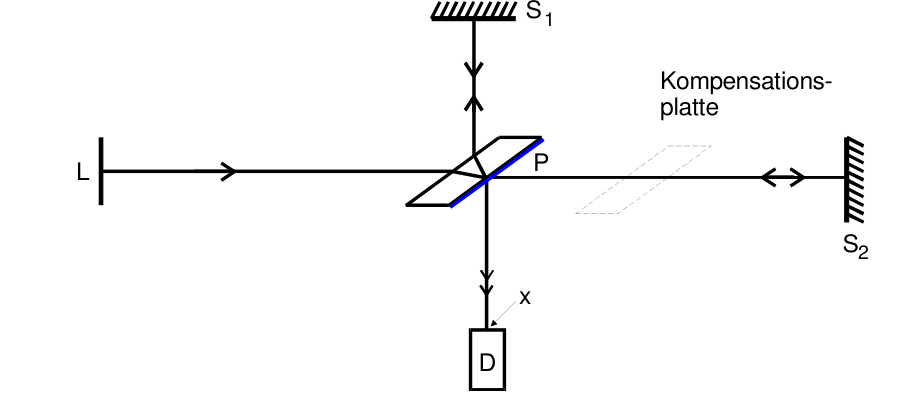
\includegraphics[width=0.9\textwidth]{18_v401/Abbildungen/Screenshot (4).png}
    \caption{Prinzipieller Aufbau des Michelson Interferometers \cite{man:v401}}
    \label{fig:schema_a}
\end{figure}
Ein Interferometer, teilt Licht in zwei Strahlen auf und führt sie wieder zusammen.
Durch die Veränderung eines der beiden Wege entsteht eine Veränderung des Interferenzmusters.
Aus dieser Veränderung können schließlich Rückschlüsse auf die Beschaffenheit der Lichtquelle gezogen werden.
Das Michelson Interferometer verwendet hierzu einen halbdurchlässigen Spiegel, der in einem \qty{45}{\degree}-Winkel 
zu dem Einfallendem Licht aufgestellt ist. 
Wie in Abbildung \ref{fig:schema_a} zu sehen wird der Lichtstrahl in zwei Arme aufgeteilt und von zwei Spiegeln wieder zurück reflektiert.
Der Strahl, der in $S_2$ reflektiert wird würde die Glasscheibe des Spiegels nur einmal durchlaufen im Gegensatz zu dem $S_1$ Strahl
der sie dreimal durchläuft.
Um einer Phasenverschiebung durch diesen Unterschied entgegenzuwirken wird eine Glasscheibe im gleichen Winkel 
auch in den Weg des $S_2$ Strahls gelegt.
Das Licht kann so am Detektor kohärent sein, wenn der Unterschied in den Weglängen der Arme kleiner der Kohärenzlänge ist.
Aus der Addition von zwei Wellen, bei der der eine Arm um d länger ist als der andere ergibt sich für die Intensität folgender Therm
\begin{align}
    I(d) = 2 \text{const} E_0^2 \left(1+ \cos\left(\frac{2\pi}{\lambda} 2d + \pi\right)\right).
\end{align}
Bei kontinuierlicher Vergrößerung um d schwankt I(d) also zwischen 0 und dem Maximalwert.
Verschiebt man den einen Spiegel in Strahlrichtung um das Stück $\Delta d$ und zählt die Anzahl der Helligkeitsmaxima $z$ ab
dann gilt folgender Zusammenhang:
\begin{align}
    \Delta d = z \frac{\lambda}{2}
    \label{eq:d_mod}
\end{align} 
Die Beschaffenheit des einen Armes kann auch durch einführung eines Materials mit unterschiedlichem Brechungsindex 
geschehen.
\begin{figure}
    \centering
    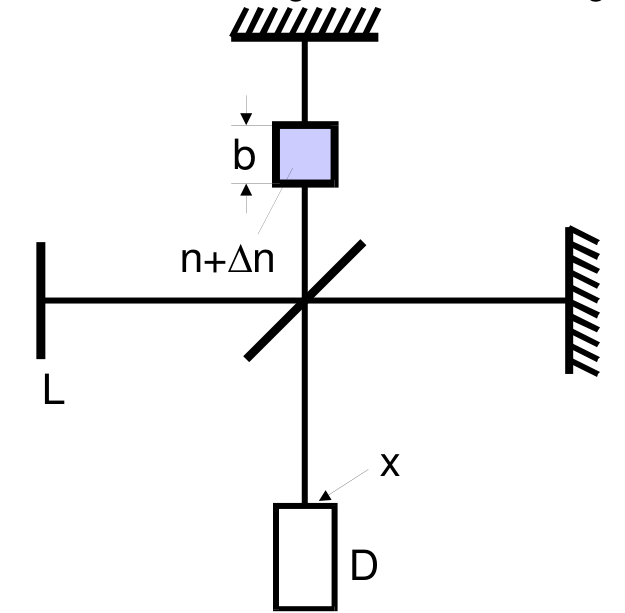
\includegraphics[width=0.4\textwidth]{18_v401/Abbildungen/Screenshot 2023-06-17 170025.png}
    \caption{Michelson-Interferometer zur Bestimmung eines Brechungsindex \cite{man:v401}}
    \label{fig:schema_b}
\end{figure}
Zum Beispiel kann die Luft aus einer Kammer (vgl. Abbildung \ref{fig:schema_b}) der tiefe $b$ herausgezogen werden,
wobei sich der Brechungsindexum $\Delta n$ verändert.
Mit $n$ als Brechungsindex der Luft und $n + \Delta n$ ergibt sich wiederum ein Gleichung für die Anzahl der Maximumsdurchläufe.
\begin{align}
    b \cdot \Delta n = \frac{z \lambda}{2}
    \label{eq:n_mod}
\end{align}
Aus der Thermodynamik und der idealen Gastheorie kann eine Gleichung für den Brechungsindex hergeleitet werden
\begin{align}
    n(p_0, T_0) = 1 + \Delta n(p, p') \frac{T}{T_0} \frac{p_0}{p-p'}.
    \label{eq:p_primed}
\end{align}
Hierbei sind $p_0$ und $T_0$ der Außendruck während der Druck in der Kammer von $p$ nach $p'$ geändert wird 
um die Änderung $\Delta n$ zu erreichen.

% Abhängigkeit von \alpha könnte hier noch rein... ist aber nicht so relevant verändert nach meinem 
% Verständnis nicht die Anzahl der Durchläufe. Außer vielleicht bei Störungen.